\documentclass[]{article}
\usepackage[]{graphicx}
\usepackage[]{xcolor}
\usepackage[]{minted}
\usepackage[utf8]{inputenc}

\begin{document}
\author{Matteo Ielacqua}
\title{Github Social}
\maketitle
    \section{Brief introduction}
    A large social network of GitHub developers which was collected from the public API in June 2019. Nodes are developers who have starred at least 10 repositories and edges are mutual follower relationships between them.
    \subsection{Context}
    GitHub is a double scope platform: In first place is used to store and develop software , either by open source developers and by companies, secondly is a social network for developers in which them can argue about technical solution and future projects. In GitHub a user can Fork ( copy the repository in his own userspace), view the code and star a repository. But is also possible to follow a developer in order to be notified on his commits on the projects he is working on, and that's what the network is collecting. The original scope of this network was to target each developer (node) and understand if it is a machine learning or web developer, the content of this information is available in the file musae\_git\_target. The network was collected using a Multiscale approach (MUSAE), the edges are mutual follower relationships between the nodes, so the network is undirected.
    
    \subsection{What to expect}
    This is a social network, so we expect a sparse graph with very few node very popular and most of them not. Most of the nodes should be part of a giant component. Triadic closure is probably given by some developers working on the same project (assumpting that the node is respecting the requirements of have starred 10 repositiories) and so we expect the presence of some big communities given by the presence of big project (like for example Unreal Engine source code or Qt company code). Sure there will a clearly manifestation of homophily, especially in those project oriented only in machine learning or webdesign, but what about bigger project that requires some exchanges of competences? The answer in obvliviously that heterophily has to be seen in those contexts. 

    \section{Basic Measures}
    
    \subsection*{Number of nodes and links}
    nodes in the network are : 37700, meanwhile links are : 289003. The dataset is indeed small, but large enough to allow some meaningful statistical measures. The network is connected, that means that there aren't disconnected subnetworks, so the largest connect component size is 37700.
    
    \subsection*{Density}
    Density is calculated using the formula $d=\frac{2L}{N(N-1)}$ where L is the number of links and N the number of nodes, this measure is taken by dividing the actual number of links on the maximum possible in this network. The result of this operation is 0.0004, such a low density is typical of social networks and this is one of them.

    \section*{Degree}   
    From a statistical view the subsequent data was obtained:
    \begin{itemize}
        \item Mean: 15.3317
        \item Max: 9458
        \item Min: 1
        \item Variance: 6526.5443
    \end{itemize}
    The average degree is indicating that most of nodes have few connection to others, comparing this measure with the maximum and the variance it's reasonable to say that there are nodes very popular while there are others quite unknown, this behaviour is in line with the social networks ones. The average degree can be used to calculate the density with the following formula $$d=\frac{<k>}{N-1}$$ where $<k>$ is the average degree and N is the total number of nodes, again the result is 0.0004 confirming that both density and average degree are correct. 

    \subsection*{Degree distribution}

    \begin{center}
        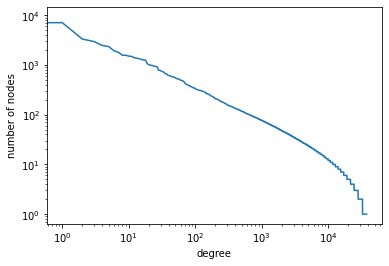
\includegraphics[scale=0.50]{charts/degree_dist_plot.png}
        \end{center}
    Plotting the histogram of degree distribution the following can be found:
    The chart clearly expose the difference in the degree distribution, mostly of the nodes are unknown but very few nodes are very popular, perhaps indicating that some power law can be present in the distribution of this measure. \\
    Using the module powerlaw from python the following chart of the cumulative distribution function (ccdf) is obtained:
    \begin{center}
    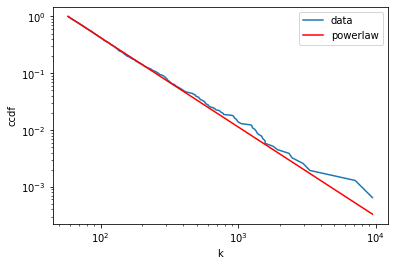
\includegraphics[scale=0.5]{charts/powerlaw.png}
    \end{center}
    In the chart the red line is the ccdf of a tipical powerlaw, meanwhile the blue line is the ccdf of the degree. Comparing the line is visible that the degree distribution is following a power law of type $f(k) \propto k^{-\alpha}$, the module also can estimate $\alpha$ that assumed the value 2.5733, meaning that the degree distribution is not only a power law but is also in the scale free regime because the exponent is in the interval [2,3].

    \section*{Assortativity Measures}
    \subsection*{Clustering Coefficient}
    The analysis of Clustering Coefficient was computer using the networkx.clustering function that just follows the formula 
    $C(i)= \frac{\tau(i)}{\tau_{\max}} = \frac{2\tau_i}{k_i(k_i-1)}$ , or in latter words the ratio between traingles present around the node i $\tau_i$ and the maximum possible value of traingles that can be around i $\tau_{\max}$ . The distribution of this measure is the following: 
    \begin{center}
        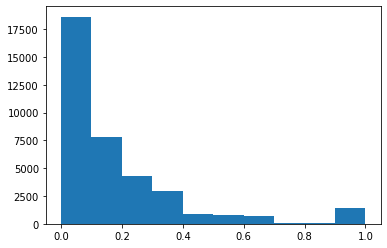
\includegraphics[scale=0.5]{charts/cc_distr.png}
    \end{center}
    It seems that over half of the nodes has no triangles, while there are very very few that have the maximum value possible. This mean that half of the nodes can perhaps be connected to the graph by a single edge, because usually we expect triadic closure to form a new edge between 2 nodes that shares the same node.
    \subsection*{Degree Correlation}
    In order to understand better assortativity, let's plot the degree correlation function using the definition of $k_{nn}(i)= \frac{1}{k_i}\sum_j(a_{ij}k_j)$ as the average degree of the neighbours of node i and $k_{nn}(k) = <k_{nn}(i)>_{i:k_i=k}$ as the average degree of neighbours of node i that have degree k.
    \begin{center}
        \includegraphics*[scale=0.5]{charts/assort_plot.png}
    \end{center}
    From the chart is evident that this network is a metabolic disassortative network,So it's a network with few spot that are connected to a great quantity of leafs as an hub and spoke shape. While it's unusual in a social network this behaviour can be caused by the architecture of Github itself, usually for big projects (like big tech companies open source releases) a user is created and contains the repositiories (we said that is the holder of repository) not only of the interested project but also plugins and third party, so when for example a Unreal Engine developer wants to download the update directly from the repository and compile it itself he follow the user proprietary of such project, in this way he will be notified if a new update has been released (this happens for example also for Tensorflow, a Tensorflow user exists and also it is the owner of the project). But in this network the edges are mutual relationships, so the hypothesis can be that leafs are employed people working on a repository, the hub are companies or user that hold that project that follow the direct contributors of the project itself, maybe in order to track the progress on theyr forks or private branch.

    \subsection*{Homophily} 
    Let's analyze the homophily between the 2 groups categorized in the network: machine network developers and web developers. The total number of ML developers are: 9739 meanwhile the number of web developers are: 27961, the number of cross edges is $8,9*10^4$, a simple formula to show if there is homophily or not is $N_{ce} < 2pq$ where N\_ce is the number of cross edges, p are ML developers and q are web developers. The number of cross edges is significantly less than 2pq= $ 2,7*10^8$ showing that homophily is in action.
    
    \section*{Distances}  
    \subsection*{Distances Distribution}
    Using BFS let's calculate the distances starting from node 0:
    \begin{center}
        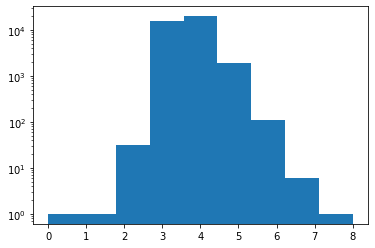
\includegraphics[scale=0.5]{charts/distances.png}
    \end{center}
    The chart show that most of the nodes have distance 4 and other significant measures are in the round of that value. Nonethless measuring the average shortest path returned a value of 4.64 so is in line with what we expected. 

    \subsection*{Centralities}
    Targeting the importance of nodes the first thing is calculate the closeness: $g_i = \frac{1}{\sum_{j!=i}l_{[ij]}}$
    \begin{center}
        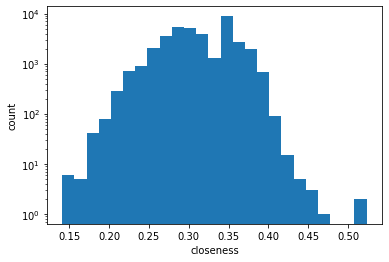
\includegraphics[scale=0.5]{charts/closeness_dist.png}
    \end{center}
    The distribution assumed by values resembled a normal distribution, with in center the mean of values:
    \begin{itemize}
        \item Mean: 0.3136
        \item Max: 0.5230
        \item Min: 0.1413
        \item Variance: 0.0016
    \end{itemize}
    Also the explicit result of those statistical values is confirming the hypothesis that the distribution is a normal like one, so the bigger part of nodes are equally closer to each other. Let's explore now the betwenness , using the estimated betwenness algorithm of the networkit package the following distribution is plotted:
    \begin{center}
        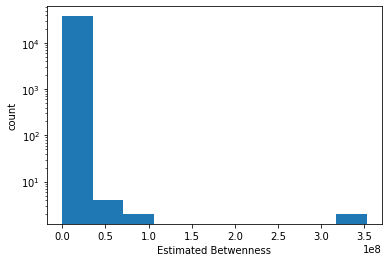
\includegraphics[scale=0.5]{charts/ebtw_dist.png}
    \end{center}
    It seems that what had been told for the closeness can be said for the betwenness, in fact most of the nodes seems to have 0 flow, meaning that no shortest path cross them at all, meanwhile there are very few nodes with the maximum value, this could mean that remove them will crash the network functionality. Let's compare the result of estimated betwenness with the exact one :
    \begin{center}
        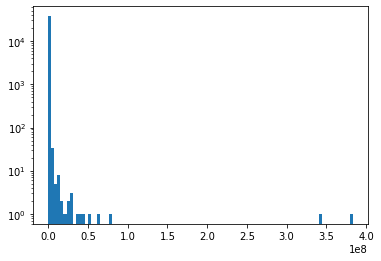
\includegraphics[scale=0.5]{charts/btw_dist.png}
    \end{center}
    the distributions are similiar, sypthom that the estimated betwenness perform quite well in estimating the value of the exact betwenness despite the lack of theoretical proof that ebtw works. Let's exploit the context to explain the causes of the behaviour of those two measures. Nodes are (for the bigger part) equally closer one to each other , this is compatible with the context, most of the nodes are employers working on common repositiories, so expect for the holders of those repositiories most of the nodes are leafs. Same could be say for the betwenness, most of the nodes aren't important at all, except for hubs of big projects, for example the maximum value of betwenness is reached in this network by node 31890 (dalinhuang99) former holder of paypaw project, a platform for exchange bitcoins (now not present anymore).

    \section*{Communities} 
    Communities where detected using the implementation brought by networkit of the Parallel Louvain Method(PLM), with refine parameter active , a gamma resolution of 1.0 and allowing the algorithm to perform till 1000 iterations. The refine parameter make the algorithm perform a second move phase to refine the parameters , the gamma resolution parameter defines the multi resolution parameter. Seeing that the algorithm yelds different results that depends on the order of visiting, it was runned multiple times taking in account the lowest possible cut size (edge cut).
    \begin{itemize}
        \item n communities            26
        \item min community size        3
        \item max community size     7883
        \item avg. community size    1450
        \item imbalance              5.43655
        \item edge cut             105214
        \item edge cut (portion)        0.364059
        \item modularity                0.461686
    \end{itemize}
    The algorithm find a remarkable number of communities considerably big in size, taking in account that each of those communities can probably represent a community of developers working on different projects, then the size can acquire a specific meaning, such that it represent the manpower at disposition for those projects. 
    Seeing that the result of the algorithm is a network composed by supernode let's also observe the graph itself.
    \begin{center}
        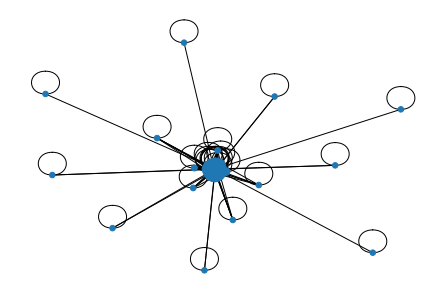
\includegraphics[scale=0.5]{charts/louvain.png}
    \end{center}
    the graph show a central big community with a lots of nodes (the self loops) connected in a hub style to all the other communities as expected from this network. Let's see how the size is distributed accross communities:

    \begin{center}
        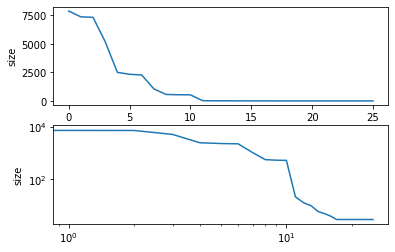
\includegraphics[scale=0.5]{charts/comm_size_dist.png}
    \end{center}
    the chart clearly show what is evident just from the graph, one very big community with other satellites less and less big, so in general a power law in this distribution is not expected.
    \begin{center}
        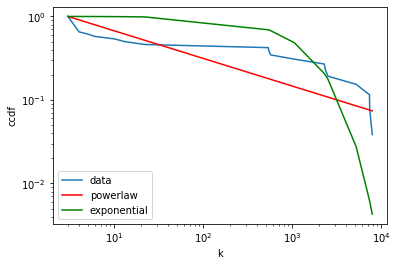
\includegraphics[scale=0.5]{charts/comms_size_powerlaw.png}
    \end{center}
    Comparing the distribution with a powerlaw and an exponential distribution is evident that none of the two approximate well the communities size distribution. 

    \subsection*{A targeted community example}
    Let's plot a community of this network, in order to obtain a viewable result a tiny community was selected.

    \begin{center}
        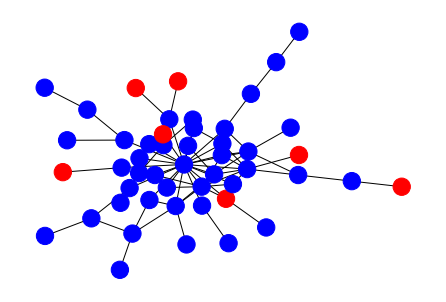
\includegraphics[]{charts/community14_graph.png}
    \end{center}
    The community is printed using the kamada\_kaway layout that is based on the kamada-kawai path-length cost function. In practice the layout is builded starting from a circular layout and then nodes are placed using kamada and kawai path length cost function. The red node in the graph represent machine learning developers, meanwhile the blue ones are web developers, using the context as an exploit to make hypothesis on this community, if perhaps the center is the holder of the project(s) maybe those are part of a web platform that involves the use of machine learning algorithms. This community in particular has 255 internal links and 135 external links, meaning that his internal link density is 0.0956. 
    
    \section*{Epidemic model}
    In order to make this model somewhat realistic let's imagine a possible scenario.
    An hacker built a virus that spread using emails, the virus will try to target the first victim and if has success in the infection will download all the emails of the GitHub users that have the highest probability to trust the email of the victim. So it will target the followers that the user follow, for each target (in random order) then it will pack itself in the email and send the email, let's assume a simple model: everytime a mail is send the victim will open it and will be infected with a probability $p(i)$, the virus target all OS (let`s assume this guy is kevin mitnick). Assuming a patch will be released $1 - p(i) = t * \frac{1}{t_{patch}}$ where t is the current step and t\_patch is the time when the patch for the virus will be released (and hopefully installed). Let's see this model implemented in python 

    \begin{minted}[]{python}

    #calculate the probability to not get infected
def notP(step, t_patch):
    return step*(1/t_patch)
    pass

    # generate a float[0,1] if lower than 1-p then get infected else not
def TossCoin(notp: float):
    return  random.random()<= 1 - notp
    pass


def PerformStep(graph: nx.graph.Graph, source: int, p: float) -> list[int]:
    infected = []
    itr = nxgraph.neighbors(source)
    for target in itr:
        if  not graph.nodes[target]["infected"] and not graph.nodes[target]["removed"]:
            if TossCoin(p):
                graph.nodes[target]["infected"] = True
                infected.append(target)
            pass
        pass
    return infected

#Custom sir model, take a node as a source of infection and a t_patch that is the time we expect the patch
def SIR(graph: nx.graph.Graph,source : int, t_patch: int) -> dict[int,list[int]]:
    frontier = []
    step = 0
    steps = {}
    frontier.append(source)
    nx.set_node_attributes(nxgraph,False,"infected")
    nx.set_node_attributes(nxgraph,False,"removed")
    while len(frontier)>0:
        nextfrontier = []
        steps[step] = []
        while len(frontier)>0:
            newt = frontier.pop()
            nxgraph.nodes[newt]["removed"] = True
            stepResult = PerformStep(graph,newt,notP(step,t_patch))
            for node in stepResult:
                nextfrontier.append(node)
                pass
            pass
        for node in nextfrontier:
            steps[step].append(node)
            frontier.append(node)
            pass
        nextfrontier.clear()
        step += 1
    return steps

    \end{minted}

    The result of running this model assuming a $t_{patch} = 100$ is this plot:
    
    \begin{center}
        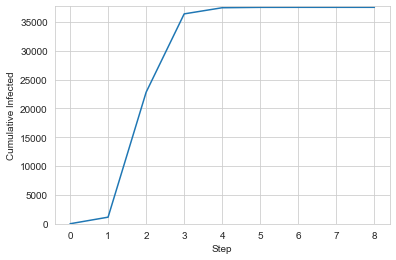
\includegraphics[scale=0.5]{charts/infection.png}
    \end{center}
    As expected given that the network is composed by hubs, when the virus approaches one of this hubs in the next step it will get a considerable number of target infected and in a few steps it will get the whole network. In cybersecurity this behaviour is observed in a real context, for example virus such Eternal Blue and Eternal Rocks infected entire companies in less than 24 hours, the peculiarity of this virus, especially of the second one, is that it replicate using a vulnerability in the smb protocol and also it send itself via email. The difference between those 2 viruses is that the second one was more dangerous, because the developer found a way to increase the hypothetic $t_{patch}$ making the virus pretending to be exactly like Eternal blue but exploiting different vulnerabilities, misleading in this way the cybersecurity researchers. The first one was immediately revealed after NSA declared that a security breach in their system allowed the thief to steal this ``tool'', so Microsoft immediately released a patch, but that is another story. Returning to the network the first chart resemble the behaviour that Eternal Rocks would have on the network, difficult to catch and analyze and it infect the whole network before any researcher can patch anything, let's make those security researchers a little bit more capable, lowering the $t_patch$ to 10 instead of 100 (Microsoft hired kevin this time), what happen?
    \begin{center}
        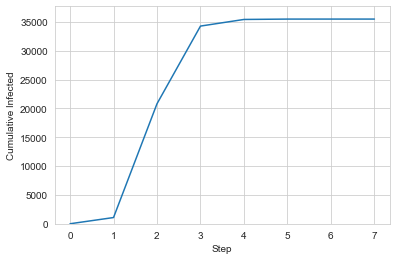
\includegraphics[scale=0.5]{charts/infection2.png}
    \end{center}
    The virus spread in the network fast enough to take most of the nodes, but not all. So the expectation is that the more $t_{patch}$ is lower the lower will be the total infected. Taking this to the limit with $t_{patch} = 2$ ,so at the second step the virus will not be able to infect anyone, the probability to infect someone will be $\frac{1}{2}$ at the step 1, not a good deal if the first target is leaf, but if is an hub for example the one with highest betwenness(31890), than in this single shot it will be able to infect on average half of the neighbors of the node, this node has 9458 neighbors.
    \begin{center}
        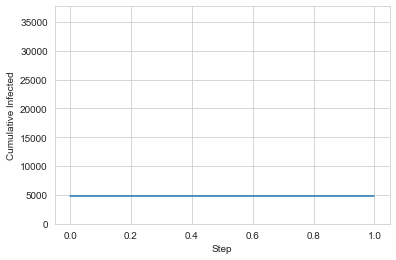
\includegraphics[scale=0.5]{charts/infection3.png}
    \end{center}
    Running the model show that the expectation is fulfilled, the virus took half of the node and stopped at the next step.

\end{document}